\documentclass{assignmeownt}

\coursenumber{CH 420}
\coursetitle{Understanding Advanced Molecular Simulation}
\title{Block 1}
\author{Qianjun Xu}
\date{}

\begin{document}
\maketitle
\thispagestyle{firststyle}

\question{Distribution of Particles}
This problem is similar to placing $n$ indistinguishable balls (particles) into $p$ distinguishable boxes (compartments in the space). The probability of finding a box has $x$ balls is
$$C_n^x(\frac{1}{p})^{x}(\frac{p-1}{p})^{n-x}$$
which follows a binominal distribution. 

\questionpart{Describe and discuss the characteristics of the distributions.}
The mode of this distribution is $(n+1)/p$. Thus when the number of compartments increases, the most common number of ball in a box decreases. As shown in Figure \ref{fig:three graphs}. In these pictures, the particle number is 64, and the number of compartments are from top to bottom 16, 32, 64, respectively.

\begin{figure}
     \centering
     \begin{subfigure}[b]{0.5\textwidth}
         \centering
         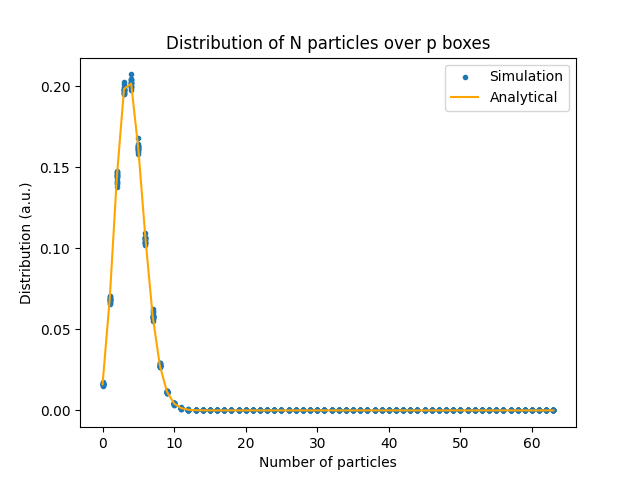
\includegraphics[width=\linewidth]{../block1/1-DistributionOfParticles/Results/64_16.png}
         \caption{$N=64,\ p=16$}
     \end{subfigure}\\
     \begin{subfigure}[b]{0.5\textwidth}
         \centering
         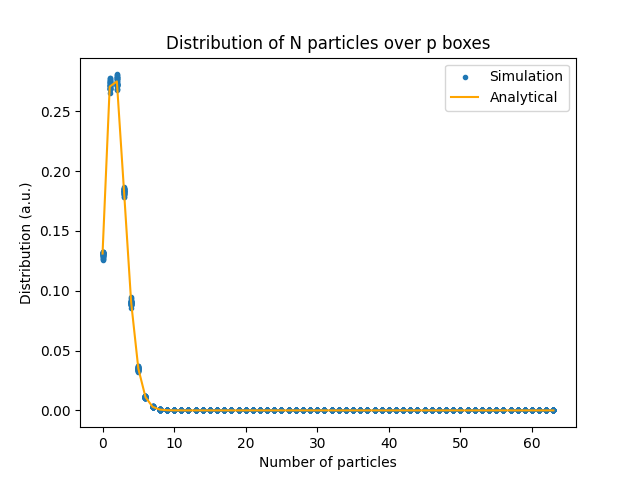
\includegraphics[width=\linewidth]{../block1/1-DistributionOfParticles/Results/64_32.png}
         \caption{$N=64,\ p=32$}
     \end{subfigure}\\
     \begin{subfigure}[b]{0.5\textwidth}
         \centering
         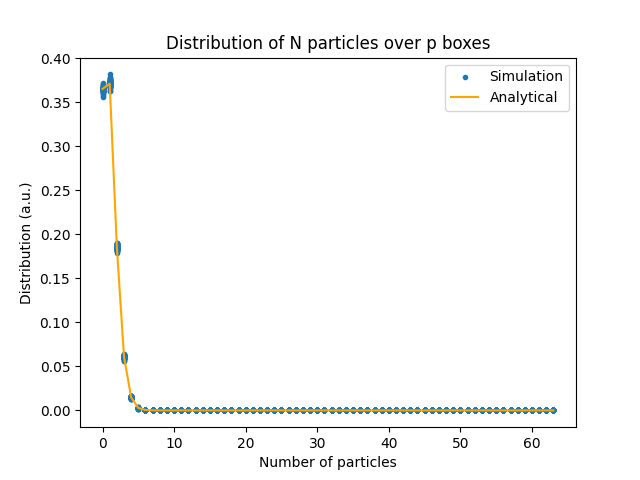
\includegraphics[width=\linewidth]{../block1/1-DistributionOfParticles/Results/64_64.png}
         \caption{$N=64,\ p=64$}
     \end{subfigure}
        \caption{Distribution of particles over boxes.}
        \label{fig:three graphs}
\end{figure}

\questionpart{Why does it (almost) never happen that one of the compartments is empty when
N/P >> 1?}
The number of ways to placing these particles into compartments is

$${n+p-1\choose n}.$$

The number of ways to ensure that at least one particle is in each compartment is

$${n+p-2\choose n}.$$

Thus the probability to find at least one empty box is

$$1-\frac{{n+p-2\choose n}}{{n+p-1\choose n}}=\frac{p-1}{n+p-1}=\frac{1}{n}\frac{p-1}{1+\frac{p-1}{n}}=\frac{p^2-2p+1}{n^2} \rightarrow 0,\ as\ n\rightarrow \infty$$

\bigskip

\question{Boltzmann Distribution}
\questionpart{Modify the problem and calculate the occupancy of each level for different values
of the temperature when all levels are non-degenerate. You can consider $\epsilon$ = 1 for
convenience. What happens at high temperatures? (Note that the temperature $T$
is expressed in reduced units, that is, $k_B$ = 1).}

The occupancy of a certain level can be calculated by

$$ O_i=\frac{g_i\times \exp{-\frac{E_i}{k_BT}}}{Q}$$

where $g_i$ is the degeneracy of energy levels, $i$ is the energy level, $E_i$ is its energy, $k_B$ is
the Boltzmann constant and $Q$ is the partition function. This is realized in Figure \ref{fig:boltzmann_modify}. When at high temperatures, we have

$$ O_i\rightarrow \frac{g_i}{Q},\ as\ T\rightarrow\infty$$

the occupancy is propotional to the degeneracy.

\begin{figure}
  \centering
  \includegraphics[]{../block1/2-BoltzmannDistribution/Results/modify_0.png}
  \caption{Calculation of occupancy for non-degenerate system.}
  \label{fig:boltzmann_modify}
\end{figure}

Thus, for the non-degenerate system, the occupancy of different level is close to the same at high temperature, as shown in Figure \ref{fig:boltzmann_rotor}.

\begin{figure}
  \centering
  \begin{subfigure}[b]{0.4\textwidth}
      \centering
      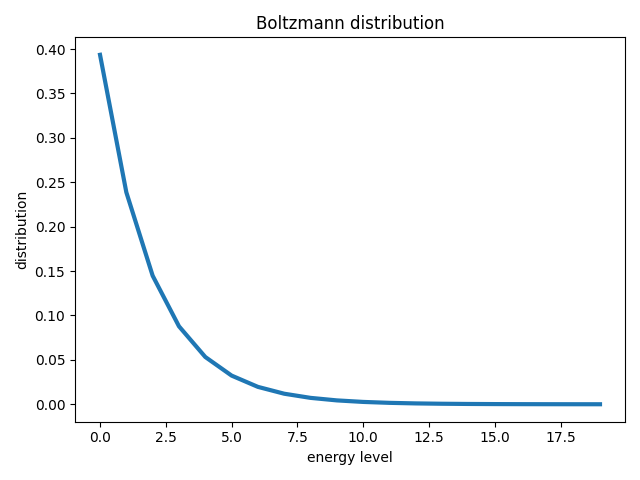
\includegraphics[width=\linewidth]{../block1/2-BoltzmannDistribution/Results/non-degeneracy/20_1.png}
      \caption{20 rotors, $T=1$}
  \end{subfigure}
  \begin{subfigure}[b]{0.4\textwidth}
      \centering
      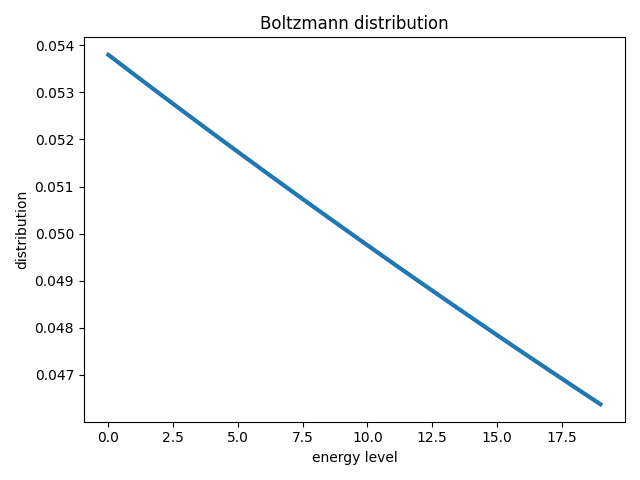
\includegraphics[width=\linewidth]{../block1/2-BoltzmannDistribution/Results/non-degeneracy/20_64.png}
      \caption{20 rotors, $T=64$}
  \end{subfigure}
     \caption{Boltzmann distribution of non-degeneracy system containing 20 rotors at different temperatures.}
     \label{fig:boltzmann_rotor}
\end{figure}


\questionpart{Change the program in such a way that the degeneracy of energy level i equals i + 1.
What do you see?}
For the degenerate system for which the degeneracy of level $i$ is $i+1$ (Figure \ref{fig:boltzmann_modify1}), the higher energy level is more occupied, as shown in Figure \ref{fig:boltzmann_rotor_degeneracy}.

\begin{figure}
  \centering
  \includegraphics[]{../block1/2-BoltzmannDistribution/Results/modify_1.png}
  \caption{Calculation of occupancy for degenerate system.}
  \label{fig:boltzmann_modify1}
\end{figure}

\begin{figure}
  \centering
  \begin{subfigure}[b]{0.4\textwidth}
      \centering
      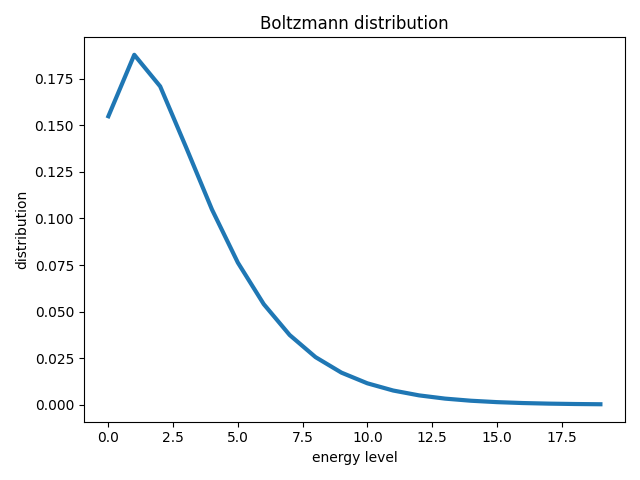
\includegraphics[width=\linewidth]{../block1/2-BoltzmannDistribution/Results/degeneracy/20_1.png}
      \caption{20 rotors, $T=1$}
  \end{subfigure}
  \begin{subfigure}[b]{0.4\textwidth}
      \centering
      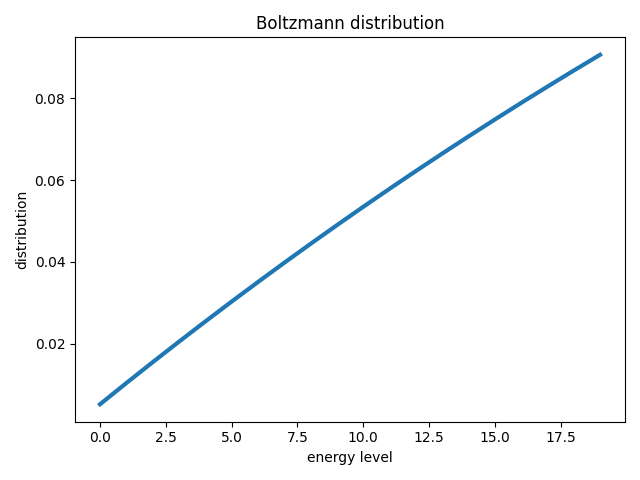
\includegraphics[width=\linewidth]{../block1/2-BoltzmannDistribution/Results/degeneracy/20_64.png}
      \caption{20 rotors, $T=64$}
  \end{subfigure}
     \caption{Boltzmann distribution of degeneracy system containing 20 rotors at different temperatures.}
     \label{fig:boltzmann_rotor_degeneracy}
\end{figure}

\questionpart{Compare your result with the approximate result for different temperatures.}

For a linear rotor, its partation function can be calculated by

$$Q=\frac{2I}{\beta\hbar^2}=\frac{2}{\beta},\ \frac{I}{\hbar^2}=1$$

which holds when $\Theta_r/T\leq 0.01$, where $\Theta_r=\frac{\hbar^2}{2I}=\frac{1}{2}$

Let's check this. The simulation is done by using the code shown in Figure \ref{fig:boltzmann_modify2}. In Table \ref{tab:partation function}, we compare the partation function calculated by the analytical expression and the partation function calculated from the simulation result. The result shown that the approximate result is close to the simulation result when $\Theta_r/T\leq 0.01$.

\begin{figure}
  \centering
  \includegraphics[]{../block1/2-BoltzmannDistribution/Results/modify_2.png}
  \caption{Calculation of occupancy for linear rotor system.}
  \label{fig:boltzmann_modify2}
\end{figure}

\begin{table}[]
  \centering
  \caption{Comparison of the partation function calculated by analytical expression and the partation function calculated from the simulation result.}
  \begin{tabular}{@{}ccc@{}}
  
  \toprule
  
  $Q_{analytical}$ & $Q_{calculated}$ & ${\Theta_r}/T$ \\ \midrule
  1   & 1.895264   & 0.5         \\
  2   & 3.118808   & 0.25        \\
  4   & 5.464034   & 0.125       \\
  8   & 9.969141   & 0.0625      \\
  16  & 18.694003  & 0.03125     \\
  32  & 35.725971  & 0.015625    \\
  64  & 69.189985  & 0.0078125   \\
  128 & 135.263539 & 0.00390625  \\
  256 & 266.198142 & 0.00195312  \\
  512 & 526.349792 & 0.000976562 \\ \bottomrule
  \end{tabular}\label{tab:partation function}
  \end{table}


\question{Coupled Harmonic Oscillators}

\questionpart{Invent a computational scheme for the update of the system at constant total energy
(U ). Compare your scheme with the scheme that is incorporated into the given
computer code (see the file harmonic.c).}

\begin{algorithm}
  \caption{Updating the system at constant total energy}
  \begin{algorithmic}
    \State Randomly select two oscillators, A and B
    \If {RandomNumber() < 0.5}
    \State A increases the energy, B decreases the energy
    \Else
    \State B increases the energy, A decreases the energy
    \EndIf
    \If {A's energy < 0 or B's energy < 0}
    \State Rollback
    \EndIf
  \end{algorithmic}
\end{algorithm}

\questionpart{Make a plot of the energy distribution (result.dat) of the first oscillator as a function
of the number of oscillators for a constant value of U/N . Which distribution is
recovered when N becomes large? What is the function of the other N -1 harmonic
oscillators? Explain.}

The energy distribution of the first oscillator recovers a Boltzmann distribution (Figure \ref{fig:boltzmann_oscillator}).

\begin{figure}
  \centering
  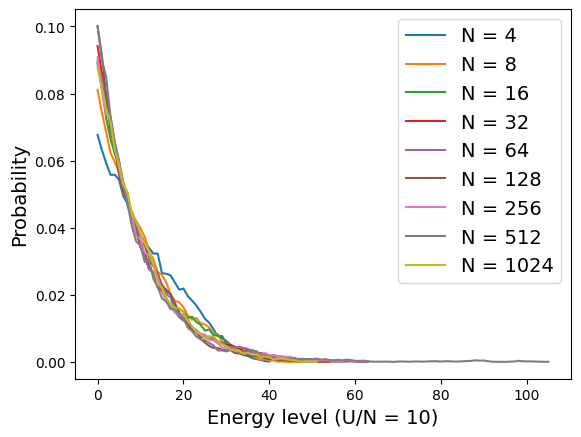
\includegraphics[width=0.5\linewidth]{../block1/3-CoupledHarmonicOscillator/Results/1.png}
  \caption{The energy distribution of the first oscillator at different number of total oscillators.}
  \label{fig:boltzmann_oscillator}
\end{figure}

The energy distribution of the others is also a Boltzmann-like distribution. It has a form

$$P(E_2) \propto \exp\{-\frac{E_1}{k_BT}\}=\exp\{\frac{E_2-E_{tot}}{k_BT}\}$$

where $E_1$ is the energy for the first oscillator and $E_2$ is the energy for the remaining (Figure \ref{fig:boltzmann_oscillator_other}).

\begin{figure}
  \centering
  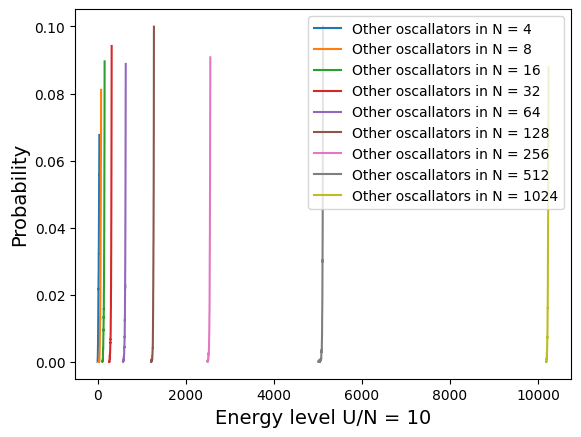
\includegraphics[width=0.5\linewidth]{../block1/3-CoupledHarmonicOscillator/Results/2.png}
  \caption{The energy distribution of the other oscillators at different number of total oscillators.}
  \label{fig:boltzmann_oscillator_other}
\end{figure}


\questionpart{Compare this distribution metioned in 2 with the canonical distribution (Use the
option NVT) of a single oscillator at the same average energy.}
The two distributions are similar (Figure \ref{fig:boltzmann_oscillator_comparison}).

\begin{figure}
  \centering
  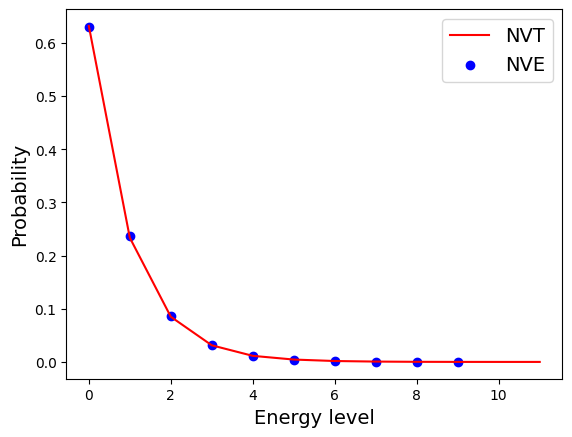
\includegraphics[width=0.5\linewidth]{../block1/3-CoupledHarmonicOscillator/Results/3.png}
  \caption{The energy distribution of the first oscillator in NVE and NVT ensemble.}
  \label{fig:boltzmann_oscillator_comparison}
\end{figure}

\questionpart{Can you explain the phenomenon you see in Question 3? How does this exercise
relate to the derivation of the Boltzmann distribution for a system at temperature
T on page 27-28 of reference1?}

This is because if we treat the first oscillator as a small system and the reservoir as a heat bath with which it can exchange energy with, the small system behaves as a NVT system and thus follows the canonical distribution.

In the derivation, we take one very small system from a large system (like here we take one oscillator from the system).

\question{Random Walk on a 1D Lattice}
\questionpart{Derive equation 5.}
To reach the position $n$ after $N$ steps, the particle must take $\frac{N+n}{2}$ steps forward and $\frac{N-n}{2}$ steps back. The number of ways to do that is

$${N \choose \frac{N+n}{2}}$$

The number of ways to take $N$ steps is $2^N$. Thus, the probability of reaching position $n$ after $N$ steps is

$$P(n, N) = \frac{N!}{2^N \frac{N+n}{2}!\frac{N-n}{2}!}$$

Take the logarithm

\begin{align*}
\ln P(n, N) = &-N\ln 2+N\ln N-\frac{N}{2}\ln(2\pi N) \\
&-\frac{N+n}{2}\ln\frac{N+n}{2}+\frac{N+n}{4}\ln\pi (N+n) \\
&-\frac{N-n}{2}\ln\frac{N-n}{2}+\frac{N-n}{4}\ln\pi (N-n) \\
=&-N\ln 2+N\ln N -\frac{N}{2}\ln 2\pi N+\frac{N}{2}\ln{4\pi}-\frac{n^2}{2N}\\
\end{align*}

Thus we have
$$ P(n, N) \propto \exp{-\frac{n^2}{2N}} $$

Normalize it, we get

$$P(n, N) = \sqrt{\frac{2}{\pi N}}\exp{-\frac{n^2}{2N}}$$

\questionpart{Run the code for a determined number of cycles and a determined number of jumps
per cycle (e.g.: 10000 cycles and 10 jumps/cycle). The code computes the distribution based on sampling, and the probability based on the equation you derived.
Plot and compare the two: are they similar?}
The simulation result (1e7 cycles, 50 steps/cycle) is plotted in Figure \ref{fig:gaussian_comparison}. According to the formula that we have derived, the expression of this gaussian is $0.2523\exp{(-\frac{n^2}{20})}$, which matches well with the simulation result.
\begin{figure}
  \centering
  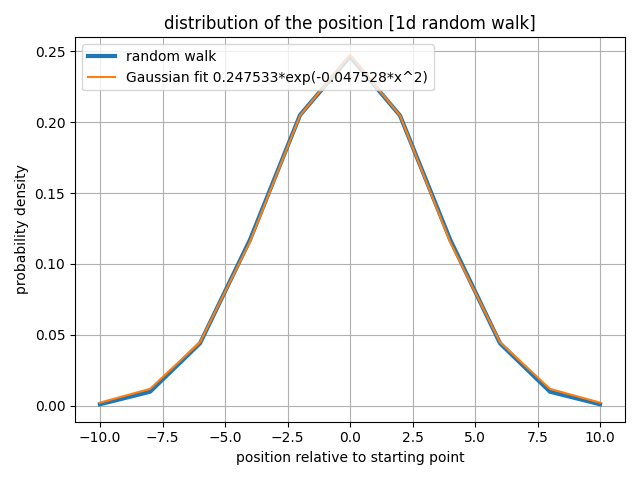
\includegraphics[width=0.5\linewidth]{../block1/4-RandomWalk1D/Results/Figure_1.png}
  \caption{The position distribution of the particle.}
  \label{fig:gaussian_comparison}
\end{figure}

\questionpart{We are now interested in the diffusivity of our system. From the concentration
profile (eq.8, see book), we can relate the mean square displacement (which can also
be computed by sampling) with the diffusion coefficient D (eq.9) in the case of 1D
(d=1). Compare the theoretical prediction in eq.9 with the numerical result you get
from running the program. What is the diffusivity of the system? (see also page
86-88 in the book, or 148-151 in the 3rd edition).}
Below is the figure of MSD versus the time. According to the theory, the MSD is propotional to the time, and the simulation result agrees with that (Figure \ref{fig:diffusivity_random_walk}). The diffusion constant is
$$
D_d = \frac{1}{2d}\lim_{t\rightarrow \infty}\frac{d}{dt}MSD(r_d)=\frac{1}{2}
$$

\begin{figure}
  \centering
  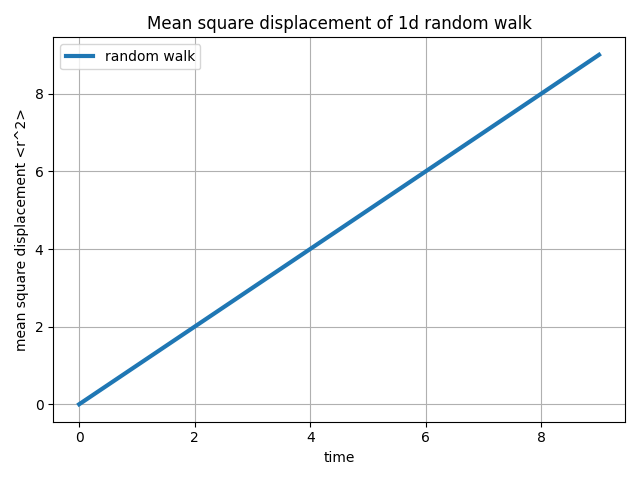
\includegraphics[width=0.5\linewidth]{../block1/4-RandomWalk1D/Results/Figure_2.png}
  \caption{The diffusivity of the particle.}
  \label{fig:diffusivity_random_walk}
\end{figure}
\questionpart{Modify the program in such a way that the probability to jump in one direction
equals 0.8. What happens?}
The result of tuning the probability of taking a move to the right to 0.8 is shown in Figure \ref{fig:diffusivity_random_walk_impeded}. You can see that the MSD curve is like a quadric curve, which means that the mean displacement is propotional to the time, and that is to say the particle has a net velocity.

\begin{figure}
  \centering
  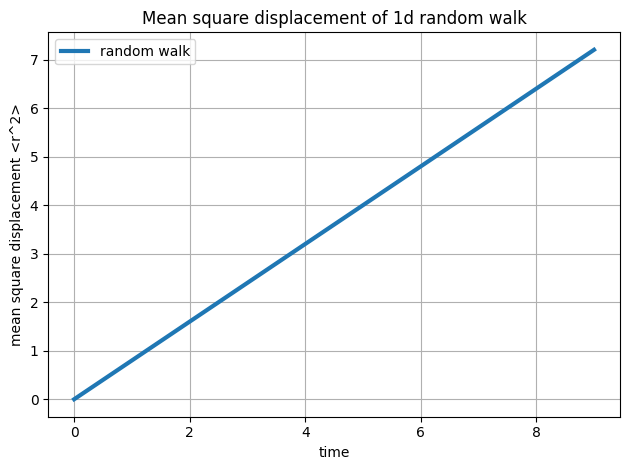
\includegraphics[width=0.5\linewidth]{../block1/4-RandomWalk1D/Results/Figure_4.png}
  \caption{The diffusivity of the particle after we modified the jump probability.}
  \label{fig:diffusivity_random_walk_impeded}
\end{figure}
\end{document}
